\documentclass[10pt,a4paper]{article}
\usepackage[utf8]{inputenc}
\usepackage[a4paper,vmargin={17mm,20mm},hmargin={20mm,20mm}]{geometry}
\usepackage{amsmath}
\usepackage{amssymb}
\usepackage{mathtools}
\usepackage{gensymb}
\usepackage{enumitem}
\usepackage{graphicx}
\usepackage{scrextend}
\usepackage{blindtext}
\usepackage{caption}
\usepackage{url}
\usepackage{subcaption}
\usepackage{circuitikz}
\usepackage{listings}
\usepackage{color}
\usepackage{natbib}
\usepackage{babel}

\definecolor{codegreen}{rgb}{0,0.6,0}
\definecolor{codegray}{rgb}{0.5,0.5,0.5}
\definecolor{codepurple}{rgb}{0.58,0,0.82}
\definecolor{backcolour}{rgb}{0.95,0.95,0.92}
\renewcommand{\baselinestretch}{1.5}
% \usepackage[a4paper, total={6in, 8in}]{geometry}

\lstdefinestyle{mystyle}{
    backgroundcolor=\color{backcolour},   
    commentstyle=\color{codegreen},
    keywordstyle=\color{magenta},
    numberstyle=\tiny\color{codegray},
    stringstyle=\color{codepurple},
    basicstyle=\footnotesize,
    breakatwhitespace=false,         
    breaklines=true,                 
    captionpos=b,                    
    keepspaces=true,                 
    numbers=left,                    
    numbersep=5pt,                  
    showspaces=false,                
    showstringspaces=false,
    showtabs=false,                  
    tabsize=2
}
 
\lstset{style=mystyle}
 

\DeclarePairedDelimiter\floor{\lfloor}{\rfloor}
\title{Final Project Report}
% \date{\today}
\sloppy
\begin{document}
\title{\textbf{Project Report - Designing HPC job schedulers using Reinforcement Learning}}
\author{
  Report by: \\
  Ishan Sharma
  \and
  Mentored by: \\
  Mr. Anirban Ghose
  \and
  Supervised by: \\
  Prof. Soumyajit Dey
}
\date{}
\maketitle

\makeatletter
\newcommand\thefontsize[1]{{#1 The current font size is: \f@size pt\par}}
\makeatother


\section{Introduction}
% \end{}
\begin{normalsize}
% \thefontsize
The project aims to develop intelligent schedulers for Embedded systems in automobiles. We consider a heterogeneous Advanced Driver-Assistance System 
\textbf{ADAS} platform comprising heterogeneous ECUs consisting both CPU and GPGPU cores and a set of object detection pipelines executing periodically to process sensor data leveraging state of the art DNNs and CNNs. There exists a natural requirement for real time guarantees for executing these object detection pipelines. The existing ADAS scheduling algorithms are not equipped to handle tasks with time varying dynamic requirements dictated by different driving contexts. Instead of investigating every possible mapping decision, an intelligent task scheduler needs to be designed which will predict task-device mapping decisions. 
\end{normalsize}

\section{Previous accomplishments}
\begin{normalsize}
The past work on the project has resulted in the development of a Discrete Event Driven Simulation Engine which acts as the environment for the reinforcement learning agent. Deep Q learning algorithm with duelling and prioritised experience replay was used to train the inference engine after prudent design of reward assignment and state extraction methodologies.
\end{normalsize}


\section{Literature Survey}
\begin{normalsize}
We now aim to develop a framework for distributed training of the Reinforcement learning agent. The general architecture consists of one or more parameter (centralised) server(s) and many worker nodes. We must decide the correct methodology of gradient updates: synchronous gradient descent, where the worker nodes pull the latest model parameters from the parameter server, acquire lock on the parameters and send the updated weights for one batch of data. The parameter server updates the weights when all workers are done with their chunk of work. \citep{chen2016revisiting} adds backup workers for to mitigate worker(s) becoming unresponsive.  On the other hand, in asynchronous gradient descent the workers can not acquire lock on the parameters which leads to the possibility of parameters becoming stale in a worker node, but downpour SGD \citep{dean2012large} found relaxing consistency requirements in practice to be remarkably effective. While the above described ways can be generally applied to any deep learning problem, \citep {ong2015distributed} outlines detailed gradient update algorithms for parameter and worker nodes. All the aforementioned works do not mention the architecture of the replay memory, which is essential to modern RL algorithms. \citep{nair2015massively} introduce Gorila and \citep{horgan2018distributed} present Ape-X architecture to address this issue with centralised replay memories accessible to both paramter and worker nodes, differing in the way replay memory is updated.

\end{normalsize}

\begin{figure}[b!]
  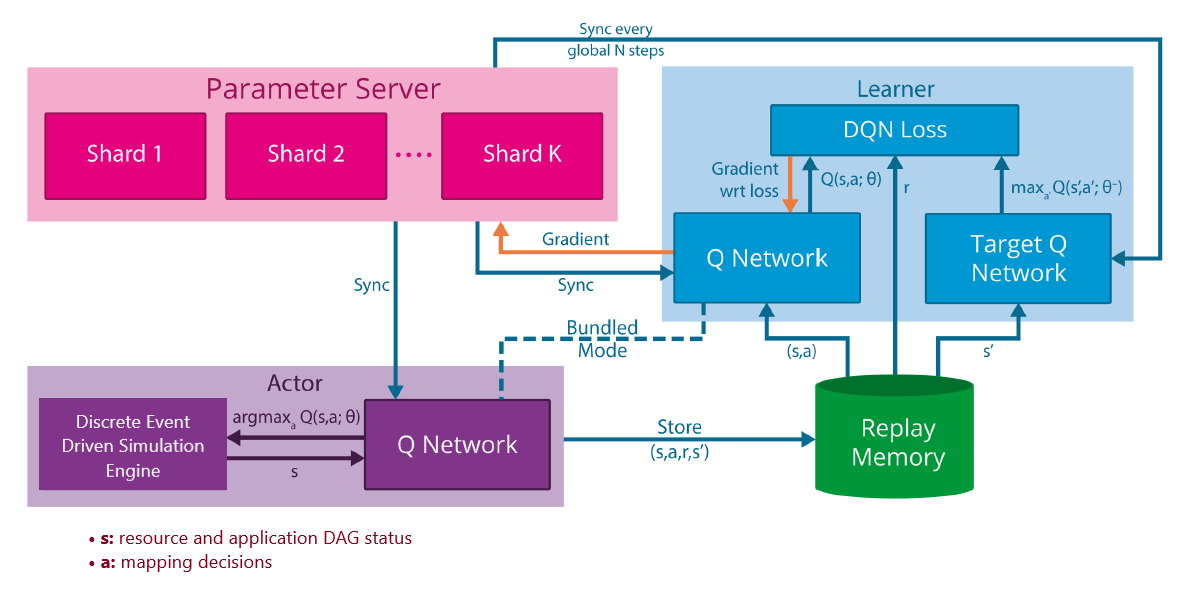
\includegraphics[width=500pt]{gorila_img.PNG}
  \caption{RL Scheduling System Overview}
\end{figure}

\section{Problems to be solved}
\begin{normalsize}
There exist \(N\) different jobs in the system. Each job can have one of \(k\) possible periods. Thus, there are \(k^N\) different period configurations. First thing to note here is that the search space is exponential in the number of jobs. Each period configuration runs for \(S\) simulations. This entire process runs for \(E\) epochs. Therefore, the entire computation is $\mathcal{O}(k^N \times S  \times E)$. Second thing to note, the search space shifts only a bit between successive period configurations. The current implementation of the RL scheduler (on one worker) relies on the learning accumulated in the previous period configurations for learning the next one. This reliance gradually increases towards the end of training. \textbf{The first problem} is how should this reliance among different period configurations to speed up the training be handled in a distributed system? \textbf{The second problem} is how should exponential decay be handled in exploration-exploitation trade-off? One of following two approaches can be followed to solve the second problem after establishing its optimality:
\begin{itemize}
    \item Distribute a proportion of \(S\) simulation runs of one period configuration among all workers at once and accumulate the results upon completion.
    \item Allot all \(S\) simulation runs of one period configuration to one worker. 
\end{itemize}
At last, we propose the following architecture (Figure 1) for RL scheduling agent's training in the distributed environment. The centralised parameter server(s) receive gradient updates from the learners and the learners synchronise their respective parameters from the parameter server(s). The replay memory is decoupled from the agent, learner, or the parameter server. The agent interacts with the Discrete Event Driven Simulation Engine (environment), with actions as mapping decisions and states as resource and application DAG status. The agent ultimately stores transition tuple in the replay memory, where the learners sample these tuples from.
\end{normalsize}

% 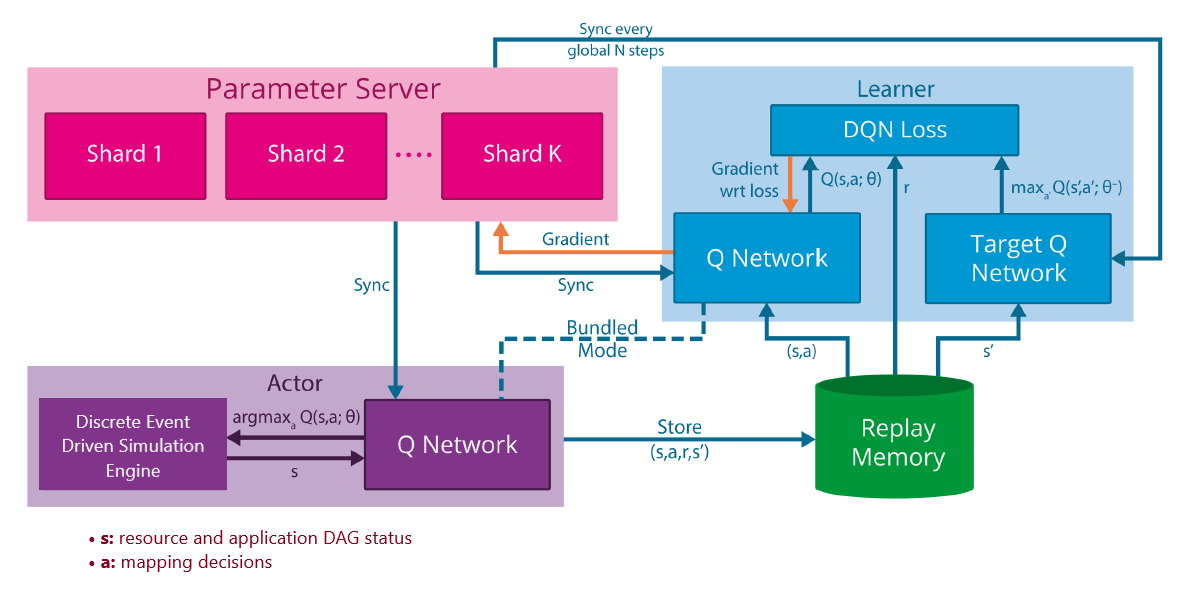
\includegraphics{gorila_img.PNG}


\clearpage
\bibliography{citations}
\bibliographystyle{rsc}
\end{document}

